
 \chapter{Special topics}\label{Special_topics}
 \section{The Reverse H\"older Inequality}\label{Reverse_holder}
 In this section, we prove the classical Reverse H\"older inequality of Gehring (cite gehring).
 
 
    Let $Q$ be a tube in $\R^n$. Let $f(x)$ be a measurable, bounded, and nonnegative function. Define the \emph{maximum function} by
\[
M(f, x)=\sup_{r>0}\,\fint_{B(x,r)} f(x) dx.
\]

In this section, we shall prove
\begin{theorem}[Reverse H\"older Inequality] Let $q>1$ such that 
\[
(M(f^q,x))^{1/q}\leq b M(f,x)
\]
a.e. $x$, where $b$ is a constant. Then there is an $\eps=\eps(n,b,q)>0$ such that 
\[
\fint_Q f^{q+\eps}(x) dx\leq C \left(\fint_Q f(x) dx\right)^{q+\eps}.
\]
\end{theorem}
 

 By rescaling, we may assume that 
 \begin{equation}\label{0}
 \fint_Q f^q(x) dx=1.
 \end{equation}
 Define
 \[
 E(t)=\{x\in Q\mid f(x)>t\}.
 \]
 

 
 We first prove the following lemma
 
 \begin{lemma}
For all $t>1$, there is a constant $a=a(n,b,q)>0$ such that 
\[
\int_{E(t)} f^q(x) dx\leq at^{q-1}\int_{E(t)} f(x) dx.
\]
\end{lemma}

\begin{proof}
Define
\[
s=\alpha t,
\]
where $\alpha>1$ is a constant to be determined. By assumption
\[
\fint_Q f^q(x) dx=1\leq s^q.
\]
We use the function $f(x)$ and the number $s^q$ to perform the \emph{Calder\'on-Zygmund
decomposition}. We then  define  a sequence of cubes $Q_j\subset Q$ such that
\begin{enumerate}
\item each side of $Q_j$ is parallel to a side of $Q$; the interior of $Q_j$ are disjoint;
\item
\begin{equation}\label{1-1-a}
s^q<\fint_{Q_j} f^q(x) dx\leq 2^n s^q.
\end{equation}
\item for \emph{a.e.} $x\not\in \bigcup_j Q_j$, we have $f(x)\leq s$.
\end{enumerate}
 Briefly speaking, the sequences can be defined inductively in the following way: we first divide $Q$ into $2^n$ sub-cubes like in Figure (ref fig2)
 
\begin{center}
\begin{tikzpicture}
   \tkzInit[xmax=1,ymax=1,xmin=-1,ymin=-1]

   \tkzGrid
 \tkzText[above](0.5,0.1){$Q'$}


  \end{tikzpicture}
  \end{center}
  %\caption{Subdivision of a cube.}\label{fig2}

 
 Let $Q'$ be one of the sub-cubes. Then
 \[
 \fint_{Q'} f^q(x) dx\leq \frac{1}{m(Q')}\int_Q f^q(x)dx\leq 2^n s^q.
 \]
 If \[
 \fint_{Q'} f^q(x) dx>s^q,
 \]
 we say $Q'$ is ``good'' and we assign $Q'$ as one of the $Q_j$'s. If $Q'$ is not ``good'', then since 
 \[
 \fint_{Q'} f^q(x) dx\leq s^q,
 \]
 we can repeat the division as above. In this way, we get a sequence $\{Q_j\}$ such that they satisfy ~\eqref{1-1-a}. Now for all $x\not\in \bigcup_j Q_j$, there is a sequence $Q_j''$ shrinking to $x$ such that
 \[
 \fint_{Q_j''} f^q(x)dx\leq s^q.
 \]
 Thus by the Lebesgue Theorem, for \emph{a.e.} $x$, $f(x)\leq s$.
 
 We define 
 \[
 G=\bigcup_jQ_j.
 \]
 Then we have
 \[
 \int_{E(s)} f^q(x) dx=\int_G f^q(x)dx=\sum_j\int_{Q_j} f^q(x) dx\leq 2^n s^q m(G).
 \]
 
 On the other hand, let $x\in Q_j$ and let $r={\rm diam}(Q_j)$. Then
 \[
 \frac{1}{m(B(x,r))}\int_{B(x,r)} f^q(x) dx\geq \frac{1}{m(B(x,r))}\, m(Q_j) s^q\geq c_1 s^q,
 \]
 where $c_1=c_1(n)>0$ is a constant. By the definition of the maximum function, we have
 \[
 M(f^q,x)\geq\fint_{B(x,r)} f^q(x) dx\geq c_1 s^q. 
 \]
 Thus by the assumption of the theorem, we have
 \[
 M(f,x)\geq (c_1/b)^{1/q} s=(c_1/b)^{1/q} \alpha t>\beta t.
 \]
 If we choose $\alpha$ large enough, we can assume that $\beta>1$. By definition of the maximum function, for any $x$, there is an $r_x>0$ such that
 \[
 \fint_{B(x,r_x)} f(x)dx\geq \beta t.
 \]
 Such a collection of balls $B(x,r_x)$ covers $Q_j$. Thus by the Vitali Covering Theorem, there is a countable subset of balls $B_j$ which are disjoint and the union of $5B_j$ covers $Q$. We therefore have the inequality
 \[
 m(G)\leq 5^n\sum_j m(B_j).
 \]
 Thus we have
 \[
 \beta tm(B_j)\leq\int_{B_j} f(x) dx\leq\int_{B_j\cap E(t)} f(x) dx+tm(B_j).
 \]
 We therefore have
 \[
 m(B_j)\leq\frac{1}{(\beta-1) t}\int_{B_j\cap E(t)} f(x) dx. 
 \]
Thus we have
\[
\begin{split}
&\int_{E(s)} f^q(x)dx\leq 2^n s^qm(G)\\
&\leq 10^n s^q\frac{1}{(\beta-1) t}\sum_j\int_{B_j\cap E(t)} f(x) dx\\&
\leq 10^n s^q\frac{1}{(\beta-1) t}\int_{ E(t)} f(x) dx.
\end{split}
\]
 On the other hand, we have
 \[
 \int_{E(t)\backslash E(s)} f^q(x) dx\leq s^{q-1}\int_{E(t)} f(x) dx.
 \]
Combining the above two inequalities completes the proof of the lemma. 

\end{proof}
 
\begin{proof}[Proof of the Reverse H\"older Inequality]
Define
\[
h(t)=\int_{E(t)} f(x) dx.
\]
Then it is easy to verify that 
\[
\int_{E(t)} f^r(x) dx=-\int_t^\infty s^{r-1} dh(s).
\]
Thus the lemma can be written as
\begin{equation}\label{2a}
-\int_t^\infty s^{q-1} dh(s)\leq at^{q-1} h(t).
\end{equation}

Define
\[
I(r)=-\int_1^\infty t^{r-1}dh(t).
\]
and for $p>q>0$, define
\[
J=(p-q)\int_1^\infty t^{p-q-1}\left(-\int_t^\infty s^{q-1}dh(s)\right) dt.
\]
Then by~\eqref{2a}, we have
\[
J\leq (p-q)\int_1^\infty at^{p-2} h(t) dt=\frac{a(p-q)}{p-1}\int_1^\infty h(t) dt^{p-1}=
\frac{a(p-q)}{p-1}(-I(1)+I(p)).
\]

On the other hand, we use integration by parts to get
\[
J=\int_1^\infty\left(-\int_t^\infty s^{q-1}dh(s)\right)dt^{p-q}=I(p)-I(q).
\]
Thus we get
\[
I(p)-I(q)\leq \frac{a(p-q)}{p-1}(-I(1)+I(p)).
\]
Thus for $p$ sufficiently close to $q$, we get
\[
I(p)\leq C(I(q)+I(1)).
\]


\end{proof}


\begin{proof}[Second Proof of the theorem] Since
\[
\int_{E(t)}f^q(x)dx\leq at^{q-1}\int_{E(t)} f(x) dx,
\]
for any $\eps>0$, we have
\[
\int_1^\infty\left(t^{\eps-1}\int_{E(t)}f^q(x)dx\right) dt\leq a \int_1^\infty\left(t^{q-2+\eps}\int_{E(t)} f(x) dx
\right).
\]
We have
\[
\begin{split}
&
LHS=\int_1^\infty\int_X t^{\eps-1}1_{\{f(x)>t\}}f^q(x) dxdt
=\int_X\int_1^\infty t^{\eps-1}1_{\{f(x)>t\}}f^q(x) dtdx\\
&=\frac{1}{\eps}\int_X (f^{q+\eps}(x)-f^q(x))dx.
\end{split}
\]
Similarly, we have
\[
RHS=\frac{a}{q-1+\eps}\int_X(f^{q+\eps}(x)-f^{q-1+\eps}(x))dx.
\]
So the theorem is proved by assuming that $\eps>0$ is sufficiently small.
\end{proof}

\begin{remark} Note that the last inequality is not homogeneous, which is fine, because we normalize the integral into~\eqref{0}.
\end{remark}




 
 \section{The Grigor'yan-Netrusov-Yau cover}\label{GNY_cover}
In this section, we give a simplified proof of (CITE GNY) {Theorem 3.5}. 

\begin{theorem}
Let a pseudo-metric space $(X,d)$ satisfy $(2,P)$-covering property. Let $m$ be a Borel measure on $X$, and assume that there exist a positive real number $v$ and $\rho$ such that 
\begin{equation}\label{1a}
\forall x\in X,\quad m(B(x,\rho/2))\leq v,\quad and\quad \exists x_0\in X, m(B(x_0,\rho))>v.
\end{equation}
Then, for any $\lambda>1$, there exists a family $\mathfrak A$ of $[\eps_0m(X)/v]$ annuli 
in $X$ satisfying the following properties
\begin{enumerate}
\item $m(A)\geq v$ for any $A\in\mathfrak A$;
\item the annuli $\{\lambda A\}_{A\in\mathfrak A}$ are disjoint. 
\end{enumerate}
Here $\eps_0$ is a number independent to $v$.
\end{theorem}






Let $N\geq 1$ be the maximum number such that 
there exists a family of annuli $\{A_i=B(x_i, r_i, R_i)\}$ with
\begin{enumerate}
\item $2C_3v>m(A_i)>C_3v$;
\item $\{\lambda A_i\}$ disjoint;
\item
\[
m(\bigcup_{i=1}^NB(x_i, 2\lambda^2 R_i))<C_1Nv
\]
for a constant $C_1>0$ independent to $v$. 
\end{enumerate}
Here $C_3$ is the constant such that when the radius is multiple by $8$, then the volume is increased by $C_3$ times. 
\vspace{.3in}

By~\eqref{1a}, we know that the family of annuli exists at least for $N=1$.\\

We shall get a contradiction by 
assuming that
\begin{equation}\label{0-0}
N<\eps_0 m(X)/v.
\end{equation}



\begin{definition}
 We say a subset 
\[
x_{i_1},\cdots, x_{i_p}
\]
of $\{x_1,\cdots, x_N\}$ is \emph{\red{admissible}}, if there are positive numbers $T_{i_j}>0$ such that 
\begin{enumerate}
\item 
\[
\bigcup_{j=1}^{p} B(x_{i_j}, \frac{1}{2\lambda}T_{i_j})\supset \bigcup_{i=1}^{N} B(x_i,   \lambda^2R_i);
\]
\item
\[
m(\bigcup_{j=1}^{p} B(x_{i_j}, T_{i_j}))\leq C_1Nv+C_2v(N-p).
\]
\end{enumerate}
\end{definition}

\begin{definition}
Let
\[
\sigma=\sup \{r\mid m(B(x,r)\backslash \bigcup_{j=1} ^p B(x_{i_j}, T_{i_j})\leq v,\quad  \forall x\in X \}.
\]
Then $\sigma<\infty$. 
We call $\sigma$ the \emph{\red{Lu's number}} with respect to the balls 
\[
B(x_{i_1}, T_{i_1}),\cdots, B(x_{i_p}, T_{i_p}).
\]
\end{definition}

Let $x\in X$ be a point such that 
\[
m(B(x,2\sigma)\backslash \bigcup_{j=1} ^p B(x_{i_j}, T_{i_j})>v.
\]

\begin{definition}
A subset, say,  $x_{i_s},\cdots, x_{i_p}$, of $x_{i_1},\cdots, x_{i_p}$ is called  \emph{\red{selected}}, if
\[
B(x,17\lambda^2 \sigma)\cap B(x_{i_j}, \frac 12 T_{i_j})\neq\emptyset
\]
for $j\geq s$. In this case, we also call $x_{i_j}$  selected if $j\geq s$, and  $B(x_{i_j}, T_{i_j})$ selected if $x_{i_j}$ is selected. 
\end{definition}


Note that there must be at least one selected ball, otherwise, we can add $B(x,3/2\sigma)$ to $\mathfrak A$, a contradiction.\\

If there are more than one selected points, say $x_{i_{p-1}}, x_{i_p}$, 
then we remove $x_{i_p}$, and replace $B(x_{i_{p-1}}, T_{i_{p-1}})$ by $$B(x_{i_{p-1}}, \max(300\lambda^3\sigma, T_{i_{p-1}}) ).$$ We claim that the new set of  balls is  still admissible. 


First, we know that
\[
m(\bigcup_{j=1}^{p-2} B(x_i,T_{i_j} )\bigcup B(x_{i_{p-1}}, 300\lambda^3\sigma))\leq C_1Nv+C_2(n-p+1)v.
\]
We shall prove
\[
 \bigcup_{j=1} ^{p-2} B(x_{i_j}, \frac{1}{2\lambda}T_{i_j})\bigcup B(x_{i_{p-1}}, 150\lambda^2\sigma)\supset
 \bigcup_{i=1}^{N} B(x_i,  \lambda^2 R_i).
 \]
 To see this 
we first observe that  
 \[
 d(x,x_{i_j})\leq 17\lambda^2\sigma+\frac 12 T_{i_j}
 \]
 for  $j=p-1,p$.
 On the other hand, 
 \[
 d(x,x_{i_j})>T_{i_j}-2\sigma
 \]
 for any $j$.
 Therefore, we have
 \[
 T_{i_j}\leq (34\lambda^2+4)\sigma,\quad d(x,x_{i_j})\leq (34\lambda^2+2)\sigma
 \]
 for $j=p-1,p$. 
Thus $B(x_{i_p}, T_{i_p})\subset B(x_{i_{p-1}}, 150\lambda^2\sigma)$, the reduced set is still admissible. \\

Using the  procedure, we can get a \emph{minimal} admissible set 
\[
B(x_1,T_1),\cdots, B(x_k, T_k).
\]

Without loss of generality, we can assume that 
\begin{equation}\label{20-2}
m(B(x_j, T_j))>C_3 v.
\end{equation}


Let $x\in X$ such that 
\[
m(B(x,2\sigma')\backslash \bigcup_{j=1} ^k B(x_{j}, T_{j}))>v,
\]
where $\sigma'$ is the Lu's number for the minimal admissible set. \\

If $B(x,2\lambda\sigma')$ doesn't touch any balls, then we can place one more ball $B(x,2\sigma')$. If $B(x,2\lambda\sigma')$ touch one of the balls, it has to touch only one of them, say, $B(x_1,T_1)$ otherwise the sequence is not minimal. 

By the above same computation
\[
T_1\leq 4(\lambda+1)\sigma',\quad d(x,x_1)\leq (4\lambda+2)\sigma'.
\]

We consider the annulus $$B(x_1,\frac 12T_1, d(x,x_1)+2\sigma').$$ 

We claim
\[
B(x_1,\frac 12T_1, d(x,x_1)+2\sigma')\supset B(x,2\sigma').
\]
To prove this, we first observe  that 
 $T_1>8\sigma'$, otherwise it contradicts to~\eqref{20-2}. 
 Let
 $z\in B(x,2\sigma')\backslash \bigcup_{j=1} ^k B(x_{j}, T_{j})$.
Then for any $y\in B(x,2\sigma')$, we have
\[
d(y,x_1)\geq d(z,x_1)-4\sigma'\geq T_1-4\sigma'\geq \frac 12 T_1.
\]
The inequality $d(y,x_1)\leq d(x,x_1)+2\sigma'$ is obvious. The claim is proved. \\


It remains to prove that the annulus 
\[
B(x_1,\frac{1}{2\lambda}T_1, \lambda(d(x,x_1)+2\sigma'))
\]
doesn't touch any other
elements in $\mathfrak \lambda A$.

To see this, we first observe that if $y\in B(x_2, \frac 12T_2)$, then 
\[
d(y, x_1)\geq d(x_2, x)-d(x, x_1)-\frac 12 T_2>17\lambda^2\sigma'-d(x,x_1)>\lambda(d(x,x_1)+2\sigma').
\]

